\chapter{Test and beam time analysis} \label{analysis}

\begin{outline}[enumerate]
\1 development of the analysis program (description of the Levenberg-Marquardt-Algorithmus.
\1 testing the analysis program with montecarlo data.
\1 Test of the detectors in the Lab.
\1 Beam line description.
\1 Data Analysis
	\2 thresholds scan
	\2 Rates on $Pb^{208}$.
	\2 Beam related asymmetry correction.
	\2 $C^{12}$ Asymmetry.
\end{outline}

\section{Model for fitting the data}
Here I have to explain the model used for describing the data, so the problem of the false asymmetry induced by variations in beam position, angle, current and energy. Here is a good point to explain the De Brujin sequence for the polarity patterns

\section{Data tree}
Explain how we compute all the values for the data tree, the position of the beam on the target, the angle, the correlated-difference values...

\section{Detectors test}
Explain the test of the two detectors in the lab, how we select the threshold, the correlation of the pmts and coincidence to select the threshold. Mention also that we observed two knees in the plot of counts vs. attenuation.

\section{Analysis}

\subsection{Alignment of the scattering plane}

\subsection{Calibration of the VFCs monitors}
Maybe it's important to divide this sections in two different part: the first part where I explain the Vfc convert the input voltage signal to a digital signal. In the second part just mention how we tuned the resistences (for X,Y monitors directly at the output signal with the oscilloscope, while for I21 and I13 monitors we used the data, so I'm able to produce plots only for the second ones).

\subsection{Calibration of the PIMO monitors}

For the calibration of the X Y monitors, we used a target made by three carbon wires placed at a certain distance from each other (that is measuered and is equal to : ...).
The position of the beam is made slowly changed first in the horizontal direction and then in the vertical direction. We observe that the pmts counts increase to a maximum, that is reached when the beam spot is centered on a carbon wire, and then decrease until the next carbon wire is hit by the beam. With a fit using a gaussian model, is possible to identify the position of the peak of the counts distribution, and from that we can directly derive the scaling factor for the XY monitors:
\begin{figure}[hbtp]
\centering
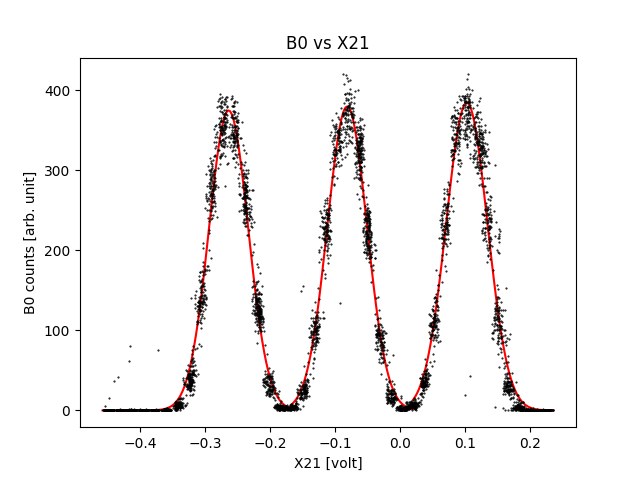
\includegraphics[width=0.7\textwidth]{Analysis/HorizontalCalibration.png}
\caption{•}
\end{figure}

\begin{figure}[hbtp]
\centering
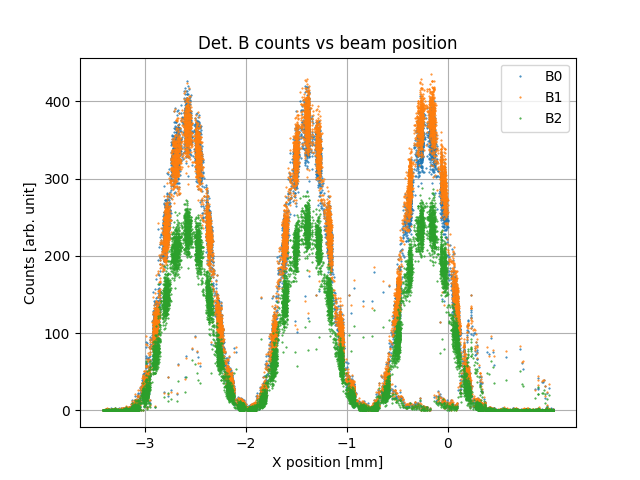
\includegraphics[width=0.45\textwidth]{Analysis/XcheckB.png} 
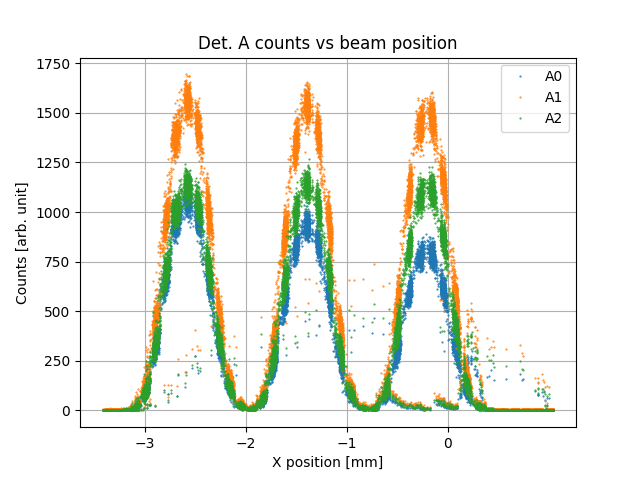
\includegraphics[width=0.45\textwidth]{Analysis/XcheckA.png}
\caption{•}
\end{figure}




\subsection{Current and ENMO monitors}

For the current monitors I13 and I21, we perform the calibration changing the current of the beam and observing the output values of the monitors (Voltage values). The we perform a fit (for the beam current, we used the nominal values that we communicate to MAMI, has the values for the x-axis).

\begin{figure}[hbtp]
\centering
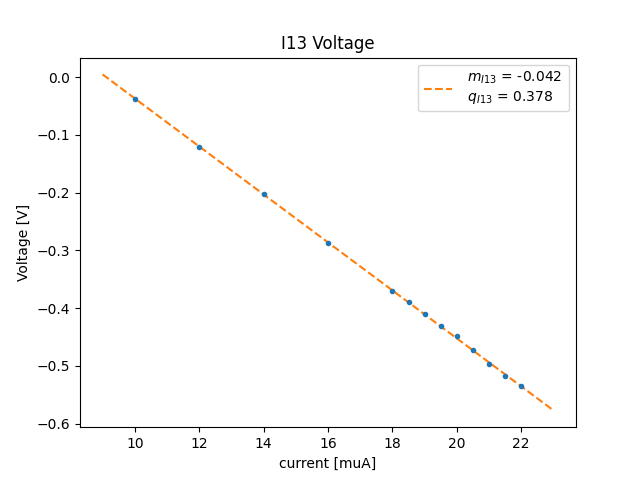
\includegraphics[width = 0.45\textwidth]{Analysis/I13_Calibration.png}
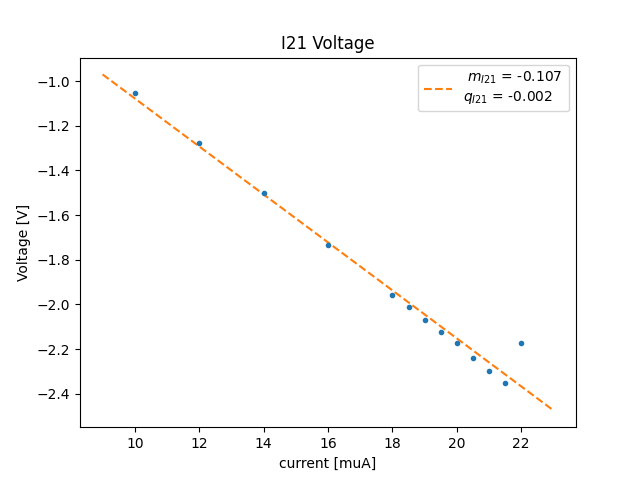
\includegraphics[width = 0.45\textwidth]{Analysis/I21_Calibration.png} 
\caption{•}
\end{figure}

For the two monitors we are able to compute the offset and scale factor:

\begin{equation}
\begin{split}
I^{volt}_{13} = m_{13} \cdot I^{Nom}_{13} + q_{13}\\
c_{13} = \frac{1}{m} \qquad offset = -\frac{q_{13}}{m}
\end{split}
\end{equation}

The same formula for current monitor I21.

The Enmo calibration is performed in a different from the other monitors. The polarity signal is sent to MAMI, and they produce a signal for the ENMO that somehow (need to investigate exactly how they do that) shows a difference between the first two subevents and the last two. This difference is equal (nominal) to $\SI{22.6}{\kilo \electronvolt}$. The idea now is to produce an histogram for the quantity $\delta E$ (with $E_{18}$ being the energy monitor):

\begin{equation*}
\delta E = \frac{E_{18}[2] + E_{18}[3]}{2} - \frac{E_{18}[0] + E_{18}[1]}{2} 
\end{equation*}

The data should be distributed with a peak around $\SI{22.6}{\kilo \electronvolt}$. To obtain the correct scaling factor for the values stored in the data tree we plot the voltage values mesured by the ENMO monitor.
3 runs of data where taken with different Beam current, to study the dependence of the measured quantity from the beam current. From the mean of the distribution it is possible to exstimate the scaling factor for the ENMO monitors, obtaining the physical quantity in the following way:

\begin{equation*}
C_{E18} = \frac{\SI{22.6}{\kilo \electronvolt}}{\overline{\delta E}}
\end{equation*}

\begin{figure}[hbtp]
\centering
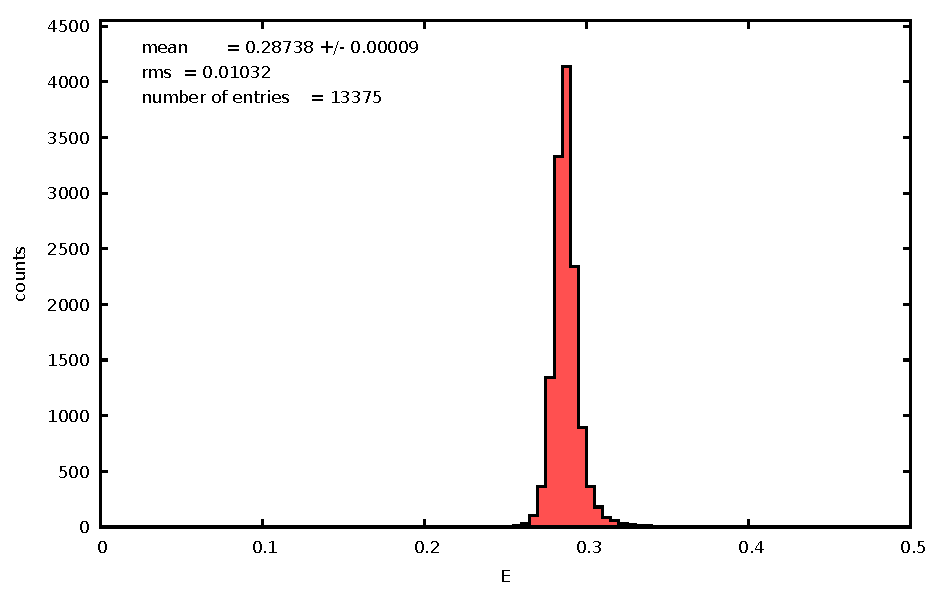
\includegraphics[width = 0.45\textwidth]{Analysis/ENMOvoltage20.pdf}
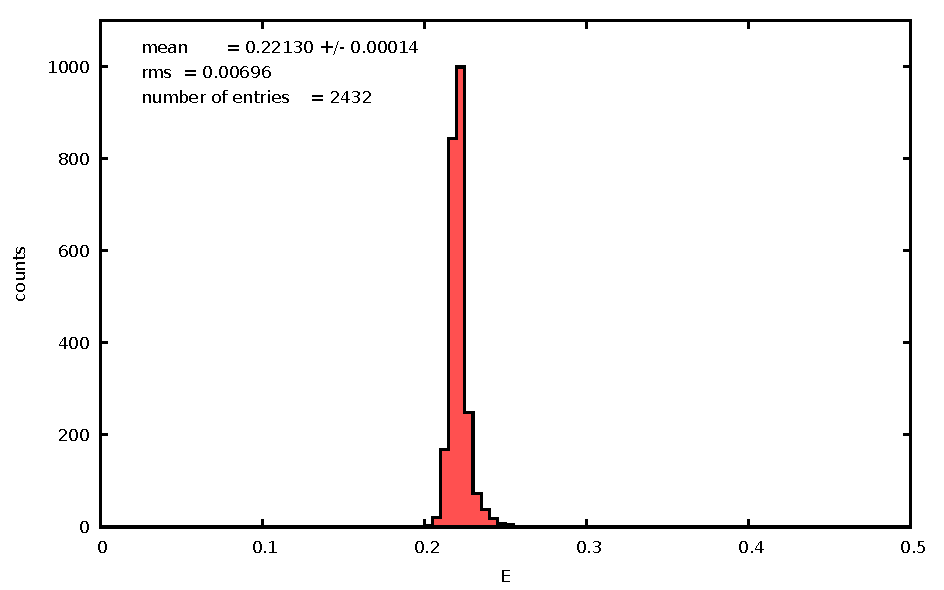
\includegraphics[width = 0.45\textwidth]{Analysis/ENMOvoltage15.pdf} 
\caption{$\delta E$ for 20 $\SI{20}{\micro \ampere}$}
\end{figure}

Taking the average over $E_{18}$ voltage values, and using the formula above, we obtain the coefficient $C_{E18}$. To take care of the current depencende of the monitors, the scaling factor to be placed in the standard.config file is: $C_{E18} \overline{I}_{\mu A}$.
The calibration was performed taking three short acquisitions with different beam current : $\SI{20}{\micro \ampere}$, $\SI{15}{\micro \ampere}$ and a run without beam. 

\begin{figure}[hbtp]
\centering
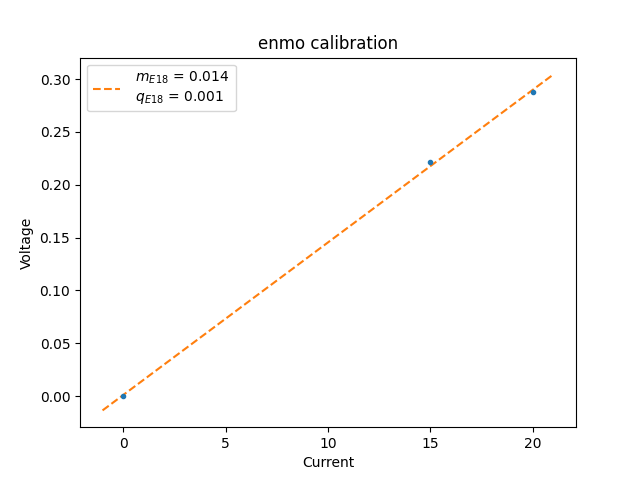
\includegraphics[width = 0.5\textwidth]{Analysis/E18_Calibration.png}
\caption{Calibration of ENMO monitor}
\end{figure}

From this we obtain the value $scaling_{E18} = -1595.2$, to obtain the physical quantity from the analysis. As a final check the final histogram for the physical quantity is shown:

\begin{figure}[hbtp]
\centering
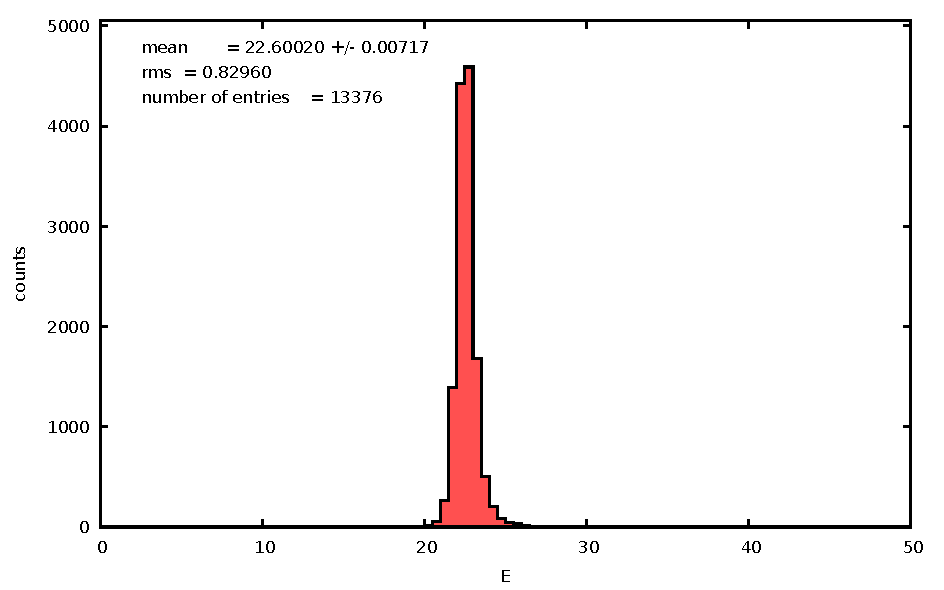
\includegraphics[width = 0.45\textwidth]{Analysis/ENMOCheck20.pdf}
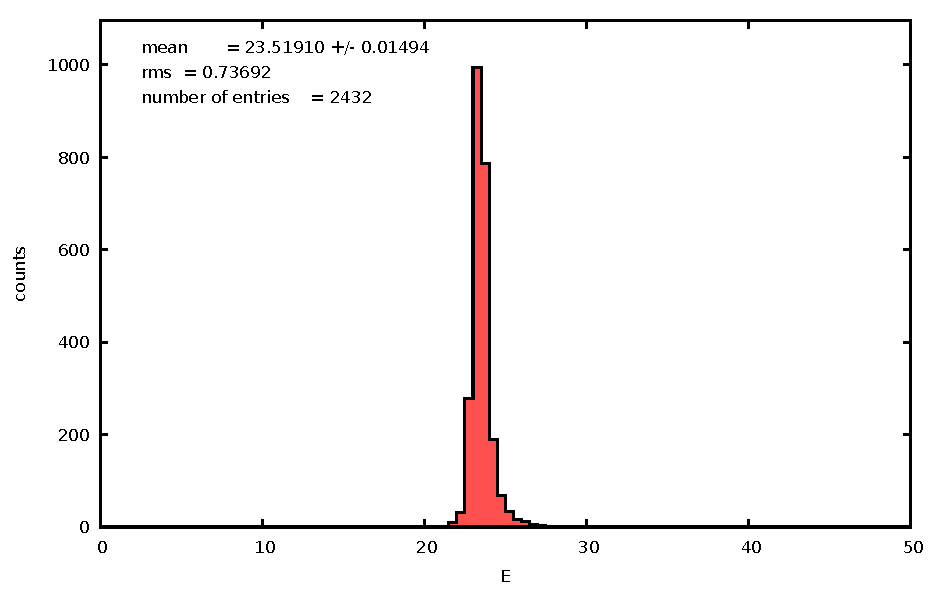
\includegraphics[width = 0.45\textwidth]{Analysis/ENMOCheck15.pdf} 
\caption{Plot for the physical quantities computed in the data tree, for two different current of the beam (on the left $\SI{20}{\micro \ampere}$, $\SI{15}{\micro \ampere}$ on the right)}
\end{figure}



\subsection{Calibration of the pmts}

Here it's important to show the plots I made during the beam time. I have to mention the Leo tecniques for the correct interpretation of counts vs attenuation.  

\subsection{Rates on lead}

This section is straightforward. Basically I have to show the single plot of the pmts counts vs. beam current for lead target. However it's possible to do some preliminary studies, for example to calculate the time needed for measuring the asymmetry on lead with a certain error and maybe check from Mott cross section that the observed rate are fine. 

\begin{figure}[hbtp]
\centering
\includegraphics[width = 0.45\textwidth]{Analysis/Rates_on_lead.png}
\includegraphics[width = 0.45\textwidth]{Analysis/Rates_on_leadB.png}
\caption{Rates on lead Target, for Detector A (left)}
\end{figure}

\section{ $^{12}C$ asymmetry}

\subsection{Autocalibration procedure}

\subsection{least square fit}

\subsection{False asymmetries}
Seems that is possible to obtain rough estimates of the beam related asymmetries with the results from the fit. For Energy and position it's achievable, while for the angles it's quite hard (in principle sounds possible to perform an analytic calculation of the asymmetry related to the incident beam angle, however Anselm told me that quite often those results are in disagrement with the observed even in the sign!).  

\subsection{??Bootstrap??}

Although Anselm was against it, now seems possible to increase the precision of the mesurement with a procedure similar to a bootstrap. Instead of computing all the quantities inside a single event, it's possible to compute all the important quantities also between different events. In this scenario the statistics can be increased artificially as mutch as we want, with the same amount of data. Of course, it's also simple to abuse of this method, so we should restrict using only events next to each other. However seem reasonable and promising.

\subsection{??interval estimation??}




